
\section{Detekcia objektu v obraze}
\label{sec:detekcia}

V prvom rade je potrebné povedať že detekcia objektu a klasifikácia v obraze je veľmi dobre známy problém v oblasti spracovania obrazu.
Pozostáva z klasifikácie obrazu do jednej z mnohých rôznych kategórií.
V dnešnej dobe už niektoré modely prebehli svojou presnosťou a výkonom aj človeka\cite{prop:NNvsHuman}.

Rozoberaním problému lokalizácie a správnej klasifikácie objektu v obraze, skončíme s potrebou
    pre detekciu a klasifikáciu niekoľkých objektou súčašne v jednej scéne.
Detekcia objektu v obraze je problém pozostavajúci z hľadania a klasifikovania variabilného počtu a rôznych typov objektov v obrázku.
Dôležitým rozdielom je "variabilná" časť. V porovnaní s klasifikáciou je výstup detekcie objektou rôznorodý svojou dĺžkou, kedže
    počet objektov v obraze sa môže meniť z obrázka na obrázok\cite{odkaz:ObjectDetectionOverview}.

\subsection{Prehľad existujúcich riešení}

\subsubsection{Klasický prístup}
Aj keď v priebehu rokov bolo množstvo rôznych typov riešení, pre túto prácu je vhodné spomenúť 2 hlavné prístupy.

Prvý z nich je Viola-Jones spôsob, ktorý navrhol v roku 2001 Paul Viola a Michael Jones v práci \cite{prop:Viola2001RobustRF}.
Tento prístup je rýchly a relatívne jednoduchý, až natoľko že sa tento algoritmus implementuje v kamerách s bodovým snímačom, ktorý umožnuje
    detekciu tvári v reálnom caše s malým množstvom potrebného výkonu.
V jednoduchosti, algoritmus generuje rôzne, môže až tisíce, jednoduché binárne klasifikátory pomocou tzv. Haar funkcií.
Tieto klasifikátory sú kaskádovito zoradené a vyhodnocované v poradí podľa ich zložitosti, s využitím viacnásobneho posuvného okna [eng. multi-scale sliding window].
V prípade negatívnej klasifikácie v ktorej koľvek úrovni vyhodnocovania, je tento proces ukončený a pokračuje sa klasifikáciou nad dalším podoknom [eng. subwindow]\cite{prop:Viola2001RobustRF}.
% TODO citacia, informacie su hlavne z https://en.wikipedia.org/wiki/Viola%E2%80%93Jones_object_detection_framework

Druhý spôsob je klasifikácia pomocou histogramu orientovaných prechodov [eng. histogram of oriented gradients] a Support Vector Machine, ktorý bude podrobne
    rozobratý v kap. \ref{sec:klasifikacia}. Tento prístup takisto používa viacnásobne posuvné okno, avšak aj keď je lepší ako Viola-Jones, je oveľa pomalší\cite{odkaz:ObjectDetectionOverview}.

\subsubsection{Prístup pomocou hlbokých neurónovych sieti}
S prípochom neurónovych sieti prišla aj veľká zmena v oblasti spracovania obrazu, preto je vhodné spomenúť niekoľko spôsob
    detekcie objektov ktoré stavajú na neurónovych sieťach.

\textbf{R-CNN} je jeden z prvých riešení \cite{prop:rcnn}, v ktorom navrhovali 3 stupňový prístup:
\begin{enumerate}
	\item[$\bullet$] extrahovať možné objekty pomocou metódy region proposal,
    \item[$\bullet$] extrahovať príznaky z každého regiónu pomocou konvolučnych neurónovych sieti,
    \item[$\bullet$] klasifikovať každý región pomocou Support Vector Machine.
\end{enumerate}

\textbf{Fast R-CNN} je označenie pre prístup ktorý vylepšil predchadzajúci R-CNN, základom je že stavia už iba na využítí konvolučnych neurónovych sieti.
V práci použili 2 prístupy k detekcii objektu, sliding window a region proposals.
Výsledky ukázali že prístup pomocou region proposal bol rýchlejší a dosiahli rýchlosť spracovania 2 snímkov za sekundu \cite{prop:fast-rcnn}.
\begin{figure}[H]
    \centering
    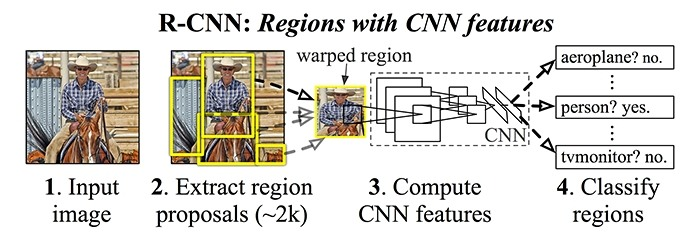
\includegraphics[width=0.8\textwidth]{rcnn}
    \qquad
    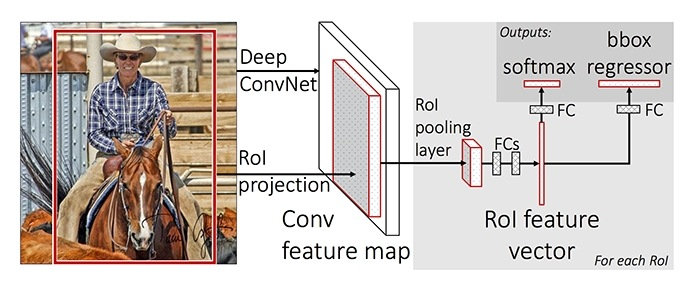
\includegraphics[width=0.6\textwidth]{fast-rcnn}
    \caption{Porovnanie architektúr R-CNN(hore) a Fast R-CNN(dole)\cite{odkaz:ObjectDetectionOverview}.}
    \label{pic:FastRCNN}
\end{figure}

\textbf{YOLO} [eng. You Only Look Once], rieši problem detekcie objektu v obraze ako regresívny problém.
Namiesto bežného postupu ako je najprv použitie region proposal techniky a následne klasifikovanie týchto regiónov.
To vedie YOLO k veľmi rýchlemu spracovaniu v reálnom čase ale za cenu presnosti.
Týmto spôsobom YOLO dokáže dosiahnuť 63.4\% mAP na 22 ms oneskorení\cite{prop:Redmon2016YouOL}.

\begin{comment}
    \subsubsection{Vyhľadávač na základe vizuálnej podobnosti obrázkov}
    Jednu z možných aplikácií detekcie objektou v obraze využíva Pinterest\footnote{\url{https://medium.com/@Pinterest_Engineering/introducing-automatic-object-detection-to-visual-search-e57c29191c30}}.
    Používaju detekciu objektou pre indexovanie rôznych častí obrázka.
    Týmto spôsobom si môže užívateľ pri hľadaní npr. špecifickej kabelky alebo topánok nájsť aj jej podobné.
    \begin{figure}[H]
        \centering
        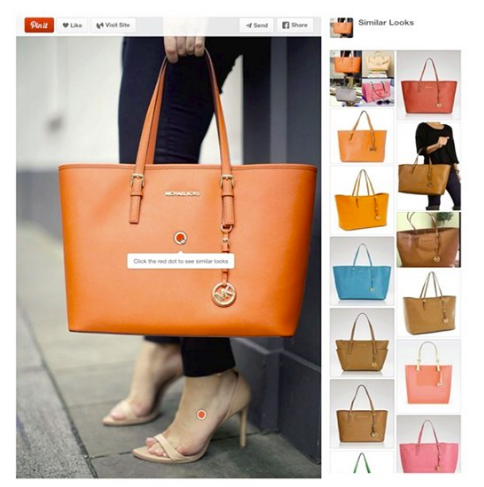
\includegraphics[width=0.5\textwidth]{purse}
        \caption{Prototyp automatického označovania a vyhľadávania objektov\cite{odkaz:ObjectDetectionOverview}}
        \label{pic:kNN}
    \end{figure}    
\end{comment}

\subsection{Kĺzajúce okno}
Kĺzajúce okno [eng. Sliding window] je jedná z metód pre detekciu objektov v obraze.
Táto metóda je veľmi vyčerpávajúca pretože zakladá na veľkom počte kandidátnych okien, až $10^4$, vo vstupnom obrázku.
Metóda prechádza vstupný obrázok na všetkých lokáciách s rôznou veľkosťou okna, následne na každom "okne" spúšta klasifikátor.
Nevýhodou tohto prístupu je jeho časová nárocnosť, preto sa tento spôsob nedá použiť pri spracovaní obrazu v reálnom čase.
Ale na druhú stranu metóda poskytuje dobrú presnosť pri kvalitnom klasifikátore\cite{prop:AutomaticHandgunDetection}.

\subsection{Regionálne návrhy}
Metóda regionálych návrhov [eng. Region proposal] na rozdiel od metódy kĺzajuceho okna, nepredpokladá za kandidátne okná všetky možnosti.
Tieto kandidátne okná su vybrané pomocou metód návrhu detekcie [eng. detecion proposel methods], konkrétne metódy
    a ich porovnanie je môžné nájsť v članku \textit{What makes for effective detection proposals?}\cite{prop:ProposalMethods}.
Prvý model na detekciu objektov ktorý použit konvolučné neurónové siete s touto metódou pre výber okien bol R-CNN\cite{prop:AutomaticHandgunDetection}.
